
\documentclass[14pt]{article}
\usepackage[utf8]{inputenc}
\usepackage[uzbek]{babel} % O'zbek tili uchun (lotin yozuvida)
\usepackage{amsmath, amssymb}
\usepackage{geometry}
\usepackage{graphicx}
\usepackage{xcolor}
\usepackage{hyperref}
\usepackage{tasks}
\usepackage{tcolorbox}
\tcbuselibrary{skins, breakable, theorems}
\usepackage{fancyhdr}
\usepackage{lastpage}
\usepackage{enumitem}
\usepackage{paracol}
\usepackage{ifthen}
\usepackage{needspace}

% Определение команд для тангенса и котангенса
\newcommand{\tg}{\operatorname{tg}}
\newcommand{\ctg}{\operatorname{ctg}}

% Настройка геометрии
\geometry{a4paper, left=10mm, right=10mm, top=20mm, bottom=20mm, headheight=15pt}

% Цветовая палитра
\definecolor{primary}{RGB}{52, 152, 219}
\definecolor{secondary}{RGB}{46, 204, 113}
\definecolor{accent}{RGB}{155, 89, 182}
\definecolor{lightbg}{RGB}{248, 249, 250}
\definecolor{taskborder}{RGB}{230, 230, 230}
\definecolor{optionbg}{RGB}{240, 242, 245}

% Основной фон страницы
\pagecolor{lightbg}

% Настройка гиперссылок
\hypersetup{
    colorlinks=true,
    linkcolor=primary,
    urlcolor=primary,
}

% Колонтитулы
\pagestyle{fancy}
\fancyhf{}
\fancyhead[L]{\textcolor{primary}{\textbf{MathCore | MOCK Test-9}}}
\fancyhead[R]{\textcolor{secondary}{Abdunazarov M.X.}}
\fancyfoot[L]{\href{https://t.me/Math_Core_Dtm_MS_Att}{\textcolor{primary}{MathCore}}}
\fancyfoot[R]{\href{https://t.me/Abd_mardon}{\textcolor{secondary}{@Abd\_mardon}}}
\fancyfoot[C]{\textcolor{gray}{\thepage/\pageref{LastPage}}}
\renewcommand{\headrulewidth}{0.5pt}
\renewcommand{\headrule}{\hbox to\headwidth{\color{primary}\leaders\hrule height \headrulewidth\hfill}}
\renewcommand{\footrulewidth}{0.5pt}
\renewcommand{\footrule}{\hbox to\headwidth{\color{secondary}\leaders\hrule height \footrulewidth\hfill}}

% Титульная страница
\title{\Huge \textbf{\textcolor{primary}{MOCK Test-9}}}
\author{\textcolor{secondary}{Abdunazarov M.X.}}
\date{}

% Стиль для карточки вопроса
\newtcolorbox{questionbox}[2][]{
    enhanced,
    breakable,
    colback=white,
    colframe=primary,
    coltitle=white,
    fonttitle=\bfseries\large,
    title={Masala \hfill \textcolor{white}{#2}},
    attach boxed title to top left={xshift=5mm, yshift=-2mm},
    boxed title style={size=small, colback=primary, sharp corners},
    sharp corners,
    boxrule=0.5pt,
    left=5mm,
    right=5mm,
    top=5mm,
    bottom=5mm,
    drop fuzzy shadow,
    #1
}

% Стиль для вариантов ответов
\newlist{options}{enumerate}{1}
\setlist[options]{
    label=\textbf{\Alph*)},
    leftmargin=*,
    itemsep=2pt,
    topsep=5pt,
    before={\vspace{2mm}\begin{tcolorbox}[
        colback=optionbg,
        colframe=white,
        sharp corners,
        boxrule=0pt,
        left=2mm,
        right=2mm,
        top=2mm,
        bottom=2mm,
    ]},
    after={\end{tcolorbox}\vspace{2mm}},
}

% Для рисунков
\newcommand{\questionimage}[2][0.5\linewidth]{%
    \begin{center}
        \includegraphics[width=#1]{#2}
    \end{center}
}

% Для удобства: команда вставки вопроса с рисунком
\newcommand{\questionitem}[4]{%
    \needspace{5cm}
    \begin{questionbox}{#1}
        #2
        \ifx&#3&%
        \else
            \questionimage{#3}
        \fi
        \begin{options}
            #4
        \end{options}
    \end{questionbox}
}

\begin{document}

% Титульная страница
\maketitle
\begin{center}
    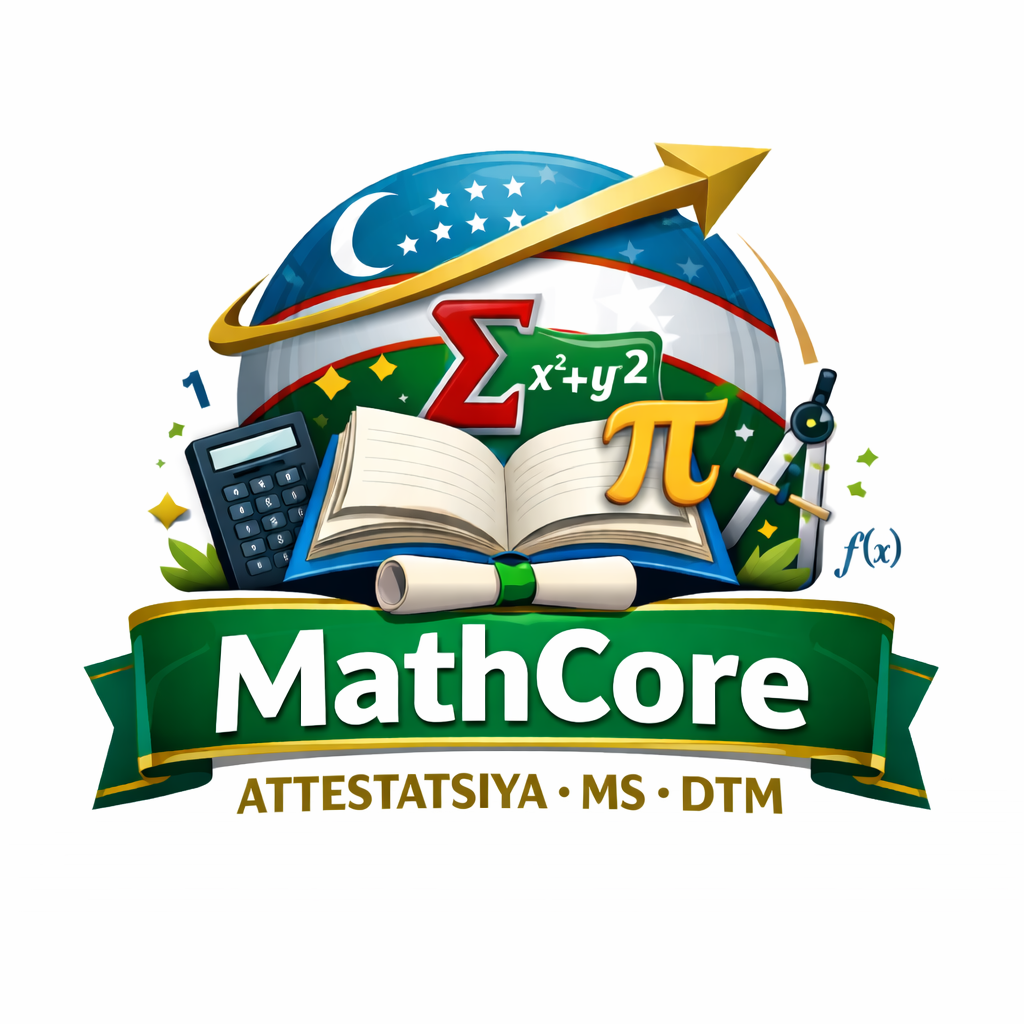
\includegraphics[width=0.2\textwidth]{logo.png} \\[5mm]
    \textcolor{gray}{\small Telegram: \href{https://t.me/Math_Core_Dtm_MS_Att}{@Math\_Core\_Dtm\_MS\_Att}}
\end{center}
\vspace{5mm}

% Masala 1
\begin{questionbox}{1}
    Quyidagi tasdiqlarning to'g'ri yoki noto'g'ri ekanligini aniqlang:
    \begin{enumerate}
        \item[(I)] \(S_n = \frac{a_1 + a_n}{4} \cdot n\) — arifmetik progressiyaning dastlabki \(n\) hadi yig'indisining formulasi.
        \item[(II)] Muntazam oltiburchakning yuzi \(S = \frac{3\sqrt{3}a^2}{2}\) formula bilan hisoblanadi, bu yerda \(a\) — oltiburchak tomoni.
        \item[(III)] Hosila: \((\arccos x)' = \frac{x}{\sqrt{1-x^2}}\).
    \end{enumerate}
    \begin{options}
        \item I – noto'g'ri, II – to'g'ri, III – to'g'ri
        \item I – noto'g'ri, II – to'g'ri, III – noto'g'ri
        \item I – to'g'ri, II – to'g'ri, III – to'g'ri
        \item I – to'g'ri, II – to'g'ri, III – noto'g'ri
    \end{options}
\end{questionbox}

% Masala 2
\begin{questionbox}{2}
    \(a + 2026\) soni 10, 12 va 15 ga qoldiqsiz bo'linadi. \(a\) ning eng kichik natural qiymatini toping.
    \begin{options}
        \item 14
        \item 8
        \item 6
        \item 4
    \end{options}
\end{questionbox}

% Masala 3
\begin{questionbox}{3}
    Uch xonali \(\overline{abc}\) va ikki xonali \(\overline{ac}\) sonlari uchun \(\overline{abc} = 7 \cdot \overline{ac}\) tenglik o'rinli. \(a + b + c\) ni toping.
    \begin{options}
        \item 6
        \item 7
        \item 10
        \item 13
    \end{options}
\end{questionbox}

% Masala 4
\begin{questionbox}{4}
    \(ABCD\) parallelogrammida \(CF\) bissektrisa, \(BE \perp AD\) o'tkazilgan. Ma'lum: \(|BC| = 9\), \(|DC| = 13\), \(|BF| = |EF| = x\). \(x\) ni toping.
    \begin{center}
        
\includegraphics[width=0.4\linewidth]{a.png}
    \end{center}
    \begin{options}
        \item 3
        \item 4
        \item 5
        \item 6
    \end{options}
\end{questionbox}

% Masala 5
\begin{questionbox}{5}
    Tengsizliklar sistemasi bilan berilgan figuraning yuzini toping:
    \[
    \begin{cases}
        x^2 + y^2 - 2x - 4y \le -1,\\
        3x - 2y + 1 \ge 0.
    \end{cases}
    \]
    \begin{options}
        \item \(2\pi\)
        \item \(3\pi\)
        \item \(4{,}5\pi\)
        \item \(9\pi\)
    \end{options}
\end{questionbox}

% Masala 6
\begin{questionbox}{6}
    \(P(x)\) ko'phad uchun \(P(3x+2) = x^2 + ax + 4\) bajariladi. \(P(x+1)\) ni \(x-4\) ga bo'lishdagi qoldiq 8 ga teng. \(a\) ni toping.
    \begin{options}
        \item 1
        \item 2
        \item 3
        \item 4
    \end{options}
\end{questionbox}

% Masala 7
\begin{questionbox}{7}
    Yarim aylanada 6 nuqta belgilangan. Tasodifiy tanlangan uchta nuqta uchburchakning uchlari bo'la olmasligi ehtimolini toping.
    \begin{center}
        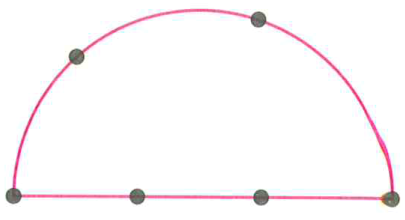
\includegraphics[width=0.4\linewidth]{dsa.png}
    \end{center}
    \begin{options}
        \item \(\frac{1}{10}\)
        \item \(\frac{1}{5}\)
        \item \(\frac{2}{5}\)
        \item \(\frac{4}{5}\)
    \end{options}
\end{questionbox}

% Masala 8
\begin{questionbox}{8}
    \(OAB\) uchburchagi \(\mathbf{a} = \overrightarrow{OA}\) va \(\mathbf{b} = \overrightarrow{OB}\) vektorlari asosida qurilgan. \(OK\) — uchburchakning bissektrisasi. \(\overrightarrow{OK}\) ni \(\mathbf{a}\) va \(\mathbf{b}\) orqali ifodalang.
    \begin{options}
        \item \(\mathbf{a}+\mathbf{b}\)
        \item \(\frac{|\mathbf{b}|\mathbf{a} + |\mathbf{a}|\mathbf{b}}{|\mathbf{a}|+|\mathbf{b}|}\)
        \item \(\frac{|\mathbf{a}|\mathbf{a} + |\mathbf{b}|\mathbf{b}}{|\mathbf{a}|+|\mathbf{b}|}\)
        \item \(\frac{\mathbf{a}}{|\mathbf{a}|} + \frac{\mathbf{b}}{|\mathbf{b}|}\)
    \end{options}
\end{questionbox}

% Masala 9
\begin{questionbox}{9}
    \(f(11{,}25^\circ)\) ni hisoblang, agar \(f(x) = \frac{\sin 6x}{\sin 2x} + \frac{\cos 6x}{\cos 2x}\).
    \begin{options}
        \item 4
        \item \(2\sqrt{2}\)
        \item 0
        \item \(-2\sqrt{2}\)
    \end{options}
\end{questionbox}

% Masala 10
\begin{questionbox}{10}
    \(OBC\) teng yonli uchburchagining (\(|OB| = |BC|\)) \(B\) uchi \(y = f(x)\) parabolasida yotadi, qolgan uchlari esa \(Oy\) va \(Ox\) o'qlarida. \(B\) nuqtasining qanday abssissasida uchburchak yuzi eng kichik bo'ladi?
    \begin{center}
        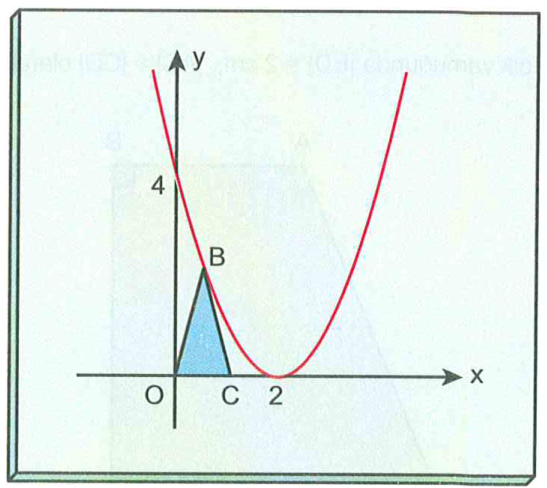
\includegraphics[width=0.4\linewidth]{aswww.png}
    \end{center}
    \begin{options}
        \item \(\frac{1}{4}\)
        \item \(\frac{1}{3}\)
        \item \(\frac{1}{2}\)
        \item \(\frac{2}{3}\)
    \end{options}
\end{questionbox}

% Masala 11
\begin{questionbox}{11}
    Tenglikdan foydalanib, \(a\) ni toping:
    \[
    \frac{x^2 + 3x}{x^3 - 2x^2 - 9x + 18} = \frac{x^2 - ax}{x^3 - 3x^2 - 4x + 12},
    \]
    \begin{options}
        \item 1
        \item \(-3\)
        \item 2
        \item \(-2\)
    \end{options}
\end{questionbox}

% Masala 12
\begin{questionbox}{12}
    \(a_1, a_2, \dots\) ketma-ketligi uchun \(a_{n+2} = a_{n+1} + a_n\) (\(n=1,2,\dots\)) bajariladi. Agar \(a_7 = 4\) bo'lsa, \(a_5 + a_8\) ni toping.
    \begin{options}
        \item 6
        \item 8
        \item 10
        \item 12
    \end{options}
\end{questionbox}

% Masala 13
\begin{questionbox}{13}
    \(\{b_n\}\) geometrik progressiya uchun ma'lum: \(b_9 - b_1 = 3\), \(b_{12} - b_4 = 24\). Progressiyaning maxrajini toping.
    \begin{options}
        \item \(0{,}(6)\)
        \item \(0{,}5\)
        \item 2
        \item 3
    \end{options}
\end{questionbox}

% Masala 14
\begin{questionbox}{14}
    Rasmda uchta to'rtburchak tasvirlangan. \(\angle NLD = 140^\circ\), \(\angle AKE = 100^\circ\). \(\angle MRF = \alpha\) ni toping.
    \begin{center}
        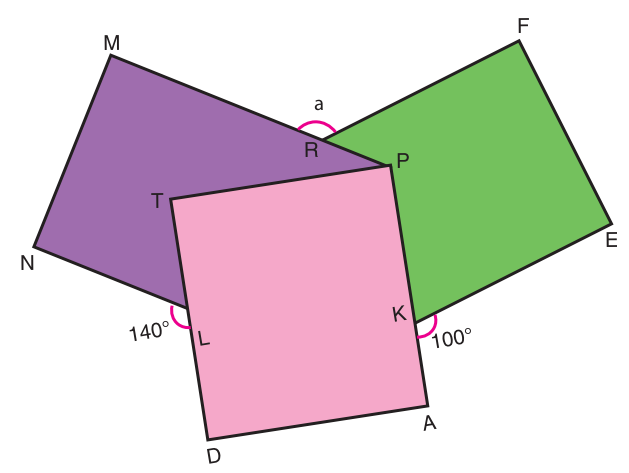
\includegraphics[width=0.4\linewidth]{hg.png}
    \end{center}
    \begin{options}
        \item \(100^\circ\)
        \item \(110^\circ\)
        \item \(120^\circ\)
        \item \(130^\circ\)
    \end{options}
\end{questionbox}

% Masala 15
\begin{questionbox}{15}
    Beshta usta ishni 20 kunda, beshta shogird esa 30 kunda bajaradi. Shu ishni 2 usta va 2 shogird necha kunda bajaradi?
    \begin{options}
        \item 30 kun
        \item 15 kun
        \item 22 kun
        \item 18 kun
    \end{options}
\end{questionbox}

% Masala 16
\begin{questionbox}{16}
    \(ABC\) to'g'ri burchakli uchburchakda: \(|AE| = |EC|\), \(|BD| = 2\), \(|AD| = 8\), \(|BC| = 6\). \(\angle ADE = x\) ni toping.
    \begin{center}
        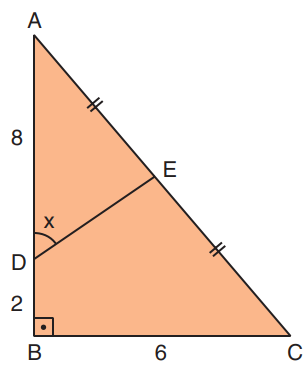
\includegraphics[width=0.3\linewidth]{fafa.png}
    \end{center}
    \begin{figure}[h]
        \centering
        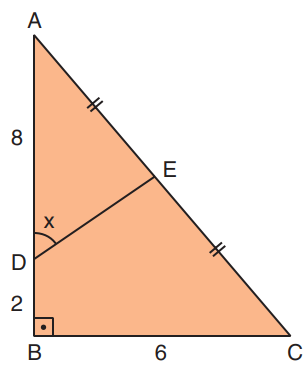
\includegraphics[width=0.4\linewidth]{fg.png}
    \end{figure}
    \begin{options}
        \item \(30^\circ\)
        \item \(45^\circ\)
        \item \(60^\circ\)
        \item \(75^\circ\)
    \end{options}
\end{questionbox}

% Masala 17
\begin{questionbox}{17}
    Hisoblang:
    \[
    \frac{\log_2 \sqrt{8} + \log_8 \sqrt{2}}{\log_2 \sqrt{8} - \log_8 \sqrt{2}}.
    \]
    \begin{options}
        \item \(\frac{5}{4}\)
        \item \(\frac{6}{5}\)
        \item \(\frac{7}{6}\)
        \item \(\frac{10}{7}\)
    \end{options}
\end{questionbox}

% Masala 18
\begin{questionbox}{18}
    \(ABCD\) to'g'ri burchakli trapetsiyada balandlik 6 ga, yon tomon katta asosga teng. Kichik asosning qanday qiymatida trapetsiya yuzi eng kichik bo'ladi?
    \begin{options}
        \item \(2\sqrt{3}\)
        \item 6
        \item \(3\sqrt{5}\)
        \item 10
    \end{options}
\end{questionbox}

% Masala 19
\begin{questionbox}{19}
    \(ABCD\) to'rtburchakda \(E\) nuqtadan tomonlarning o'rtalari \(K, L, M, N\) ga kesmalar o'tkazilgan, ular to'rtburchakni to'rt qismga ajratadi. Doiralar ichidagi sonlar yuzlarni bildiradi. \(S\) ni toping.
    \begin{center}
        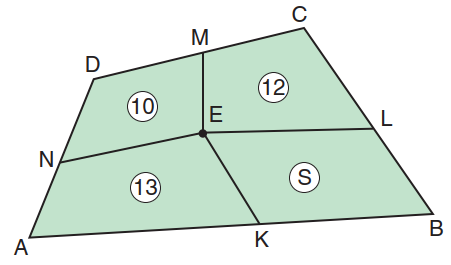
\includegraphics[width=0.4\linewidth]{qda.png}
    \end{center}
    \begin{figure}[h]
        \centering
        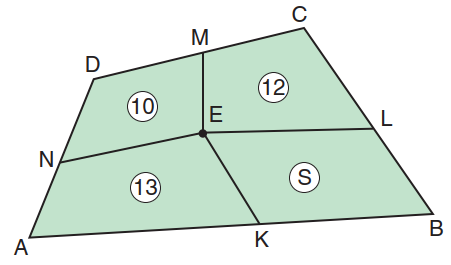
\includegraphics[width=0.4\linewidth]{we.png}
    \end{figure}
    \begin{options}
        \item 12
        \item 13
        \item 14
        \item 15
    \end{options}
\end{questionbox}

% Masala 20
\begin{questionbox}{20}
    Turli haqiqiy \(m\) va \(n\) sonlari uchun \(n^2 f(m) = m^2 f(n)\) bajariladi. \(\frac{f(3)-f(1)}{f(4)}\) ni toping.
    \begin{options}
        \item \(\frac{1}{8}\)
        \item \(\frac{1}{2}\)
        \item \(\frac{5}{8}\)
        \item \(\frac{3}{4}\)
    \end{options}
\end{questionbox}

% Masala 21
\begin{questionbox}{21}
    \(f(x) = \frac{1}{x} + \frac{1}{x^2} + \frac{1}{x^3} + \dots + \frac{1}{x^n}\) bo'lsin. Agar \(f'(1) = -66\) bo'lsa, \(n\) ni toping.
    \begin{options}
        \item 9
        \item 10
        \item 11
        \item 12
    \end{options}
\end{questionbox}

% Masala 22
\begin{questionbox}{22}
    Bir xil quvvatga ega ikkita nasos hovuzni 20 soatda to'ldiradi. Agar birinchi nasosning quvvati 20\% ga kamaytirilsa, ikkinchi nasosning quvvati 60\% ga oshirilsa, hovuz necha soatda to'ldi?
    \begin{options}
        \item 35
        \item 30
        \item 32
        \item \(\frac{50}{3}\)
    \end{options}
\end{questionbox}

% Masala 23
\begin{questionbox}{23}
    \(ABCD\) trapetsiyasida \(EF\) — o'rta chiziq. \(S_{ETK} : S_{KF} = 3 : 2\). \(KF : EK\) ni toping.
    \begin{center}
        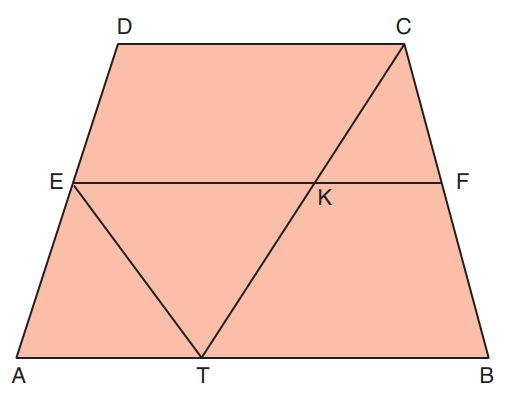
\includegraphics[width=0.3\linewidth]{rew.png}
    \end{center}
    \begin{options}
        \item \(\frac{3}{2}\)
        \item \(\frac{4}{3}\)
        \item \(\frac{2}{3}\)
        \item \(\frac{3}{4}\)
    \end{options}
\end{questionbox}

% Masala 24
\begin{questionbox}{24}
    Tengsizlikni yeching:
    \[
    \log_{\frac{1}{3}} \bigl( \log_2 (2 - x) \bigr) + 1 \ge 0.
    \]
    \begin{options}
        \item \([-6; 1)\)
        \item \([-6; 2)\)
        \item \([-6; 2) \cup (2; \infty)\)
        \item \((1; 2)\)
    \end{options}
\end{questionbox}

% Masala 25
\begin{questionbox}{25}
    Agar \(f(x) = -\dfrac{2}{x}\) bo'lsa, \(y = f(x+2) + 1\) funksiyasini toping.
    \begin{options}
        \item \(y = -\dfrac{x}{x+2}\)
        \item \(y = \dfrac{1}{x+2}\)
        \item \(y = \dfrac{2x}{x+2}\)
        \item \(y = \dfrac{x}{x+2}\)
    \end{options}
\end{questionbox}

% Masala 26
\begin{questionbox}{26}
    \([0; \pi]\) kesmasida tengsizlikni yeching:
    \[
    \sin^2 x < \cos^2 x - \frac{\sqrt{3}}{2}.
    \]
    \begin{options}
        \item \(\left[0; \frac{\pi}{12}\right) \cup \left(\frac{11\pi}{12}; \pi\right]\)
        \item \(\left(\frac{\pi}{12}; \frac{11\pi}{12}\right)\)
        \item \(\left[0; \frac{5\pi}{12}\right]\)
        \item \(\left[0; \pi\right]\)
    \end{options}
\end{questionbox}

% Masala 27
\begin{questionbox}{27}
    \(ABCD\) parallelogrammida: \(|EF| = |FB|\), \(|DF| = |FT| = |TC|\), \(|CL| = |LB|\). Sariq sohaning yuzi 8 ga teng. Ko'k sohaning yuzini toping.
    \begin{center}
        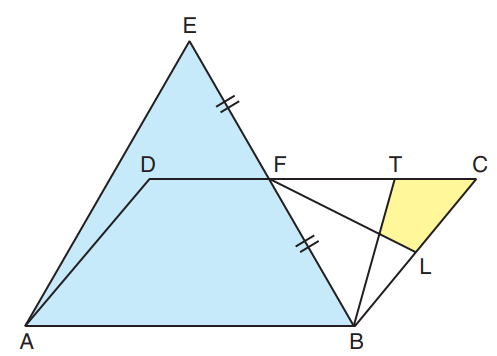
\includegraphics[width=0.4\linewidth]{равр.png}
    \end{center}
    \begin{options}
        \item 72
        \item 60
        \item 48
        \item 36
    \end{options}
\end{questionbox}

% Masala 28
\begin{questionbox}{28}
    Tenglamani yeching va uning eng kichik musbat ildizini ko'rsating:
    \[
    2\sin^2\left(x + \frac{\pi}{6}\right) + 3\sin\left(x + \frac{\pi}{6}\right) - 2 = 0.
    \]
    \begin{options}
        \item \(\frac{\pi}{6}\)
        \item \(\frac{\pi}{4}\)
        \item \(\frac{2\pi}{3}\)
        \item \(\frac{3\pi}{4}\)
    \end{options}
\end{questionbox}

% Masala 29
\begin{questionbox}{29}
    \(ABC\) uchburchakda \(BD\) — bissektrisa, \(|BE| = 3|ED| = 9\). \(|DC| = x\) ni toping.
    \begin{center}
        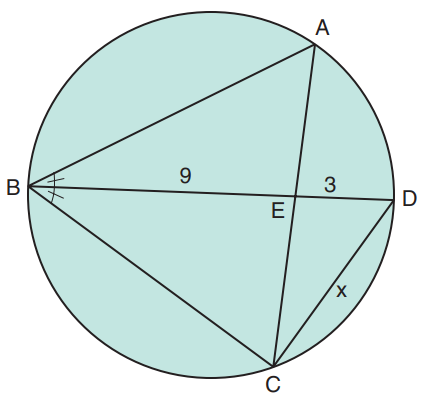
\includegraphics[width=0.4\linewidth]{fafw.png}
    \end{center}
    \begin{options}
        \item 9
        \item 8
        \item 7
        \item 6
    \end{options}
\end{questionbox}

% Masala 30
\begin{questionbox}{30}
    Sxemaga ko'ra, \(A\) nuqtadan \(C\) nuqtaga necha xil usulda borish mumkin?
    \begin{center}
        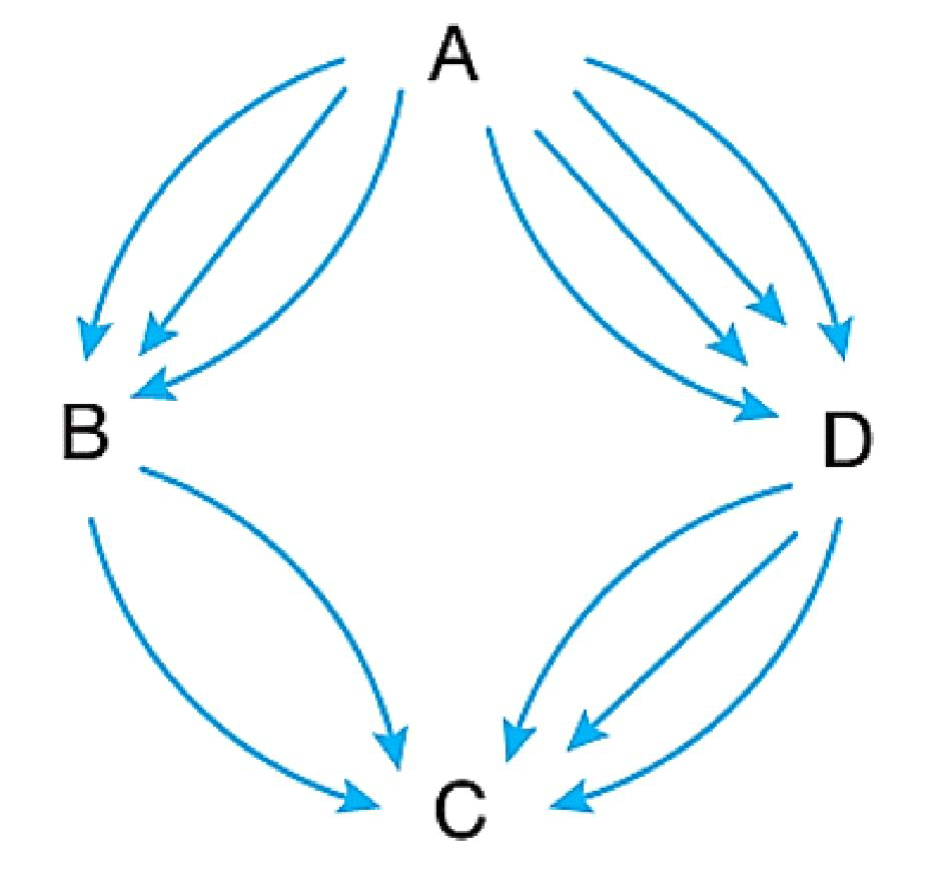
\includegraphics[width=0.4\linewidth]{ert.png}
    \end{center}
    \begin{options}
        \item 12
        \item 14
        \item 16
        \item 18
    \end{options}
\end{questionbox}

% Masala 31
\begin{questionbox}{31}
    Tomoni 4 bo'lgan muntazam oltiburchak \(ABCDEF\). Uning ichida oltiburchak uchlarida markazlari bo'lgan aylana yoylari chizilgan. Yashil sohaning yuzini toping.
    \begin{center}
        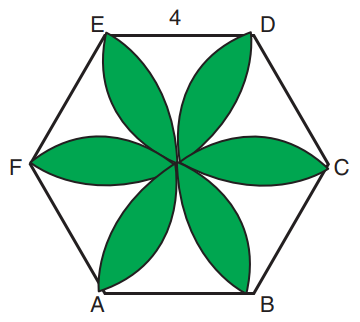
\includegraphics[width=0.4\linewidth]{232er.png}
    \end{center}
    \begin{options}
        \item \(16\pi - 32\sqrt{3}\)
        \item \(32\pi - 36\sqrt{3}\)
        \item \(24\pi - 32\sqrt{3}\)
        \item \(32\pi - 48\sqrt{3}\)
    \end{options}
\end{questionbox}

% Masala 32
\begin{questionbox}{32}
    Aniqmas integralni hisoblang:
    \[
    \int 4x \cdot \ln(3x) \, dx.
    \]
    \begin{options}
        \item \(2x^2 \ln(3x) - x^2 + C\)
        \item \(x^2 \ln(3x) - 2x^2 + C\)
        \item \(2x^2 \ln(3x) - 2x^2 + C\)
        \item \(4x^2 \ln(3x) - x^2 + C\)
    \end{options}
\end{questionbox}

% Masala 33
\begin{questionbox}{33}
    Rasmda hammom jihozlarining parallel taxtalari tasvirlangan. Birinchi, ikkinchi va uchinchi taxtalar yotadigan to'g'ri chiziqlarning tenglamalari: \(d_1\), \(d_2\), \(d_3\). \(d_1\) va \(d_2\) orasidagi masofaning \(d_2\) va \(d_3\) orasidagi masofaga nisbatini toping.
    \begin{center}
        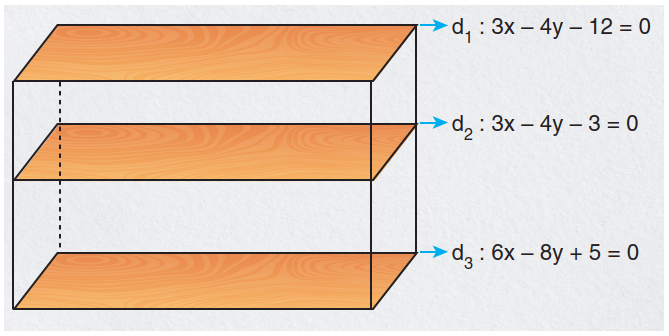
\includegraphics[width=0.4\linewidth]{tw.png}
    \end{center}
    \begin{options}
        \item \(\frac{10}{11}\)
        \item \(\frac{12}{11}\)
        \item \(\frac{16}{11}\)
        \item \(\frac{18}{11}\)
    \end{options}
\end{questionbox}

% Masala 34
\begin{questionbox}{34}
    Chizmada \(|AB| = 5\), \(|BC| = 6\), \(|EF| = 2\), \(|FG| = 3\). Qizil karton \(d\) to'g'ri chizig'i atrofida \(360^\circ\) aylantirilmoqda. Hosil bo'lgan jismning hajmini toping.
    \begin{center}
        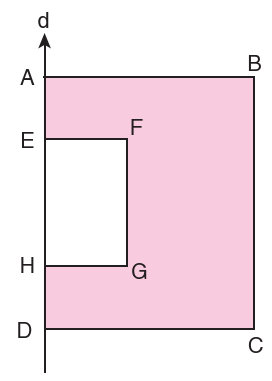
\includegraphics[width=0.4\linewidth]{5tr.png}
    \end{center}
    \begin{options}
        \item \(148\pi\)
        \item \(168\pi\)
        \item \(138\pi\)
        \item \(128\pi\)
    \end{options}
\end{questionbox}

% Masala 35
\begin{questionbox}{35}
    \(10x^3 - 39x^2 + 29x - 6\) ko'phadning ildizlari to'g'ri burchakli parallelepipedning uzunligi, eni va balandligiga teng. Parallelepipedning har bir qirrasi 2 birlikka uzaytirildi. Hosil bo'lgan parallelepipedning hajmini toping.
    \begin{options}
        \item 20
        \item 24
        \item 30
        \item 36
    \end{options}
\end{questionbox}

\end{document}